\chapter{Marco Conceptual}
\label{MarcoConceptual}

\section{SOA y WSDL}
\label{MarcoConceptual:SOA_WSDL}

\section{Gobernanza en SOA}
  \label{MarcoConceptual:GobernanzaSOA}

  La \emph{gobernanza en arquitecturas orientadas a servicios (SOA)}, es la tarea de administración de una SOA: brinda las reglas para la toma de decisiones, establece los procesos necesarios, define los roles que forman parte del sistema administrativo y establece las métricas que determinan el ajuste de la toma de decisiones a las reglas establecidas. La gobernanza no dice cuándo ni cómo tomar una decisión; determina quién debería hacerlo y establece los límites para esa persona o grupo. \cite{Erl:2011:SGG:1983453}

  \begin{figure}[h]
    \centering
    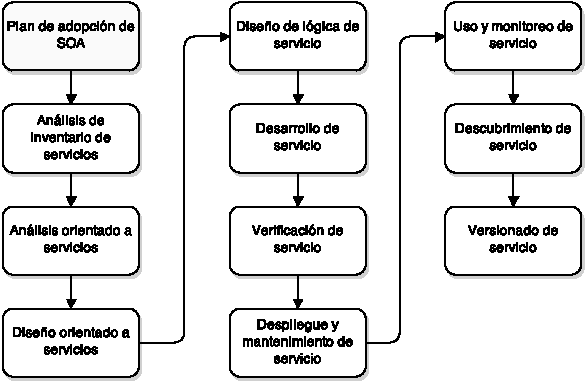
\includegraphics[width=\linewidth]{ciclo_de_vida_del_proyecto}
    \caption{Etapas comunes de un proyecto SOA}
    \label{figura:ciclo_de_vida_del_proyecto}
  \end{figure}

  La figura \ref{figura:ciclo_de_vida_del_proyecto} muestra las etapas comunes de un proyecto SOA las cuales son también etapas del \emph{ciclo de vida} de los servicios.

  Todo proyecto SOA comienza con un plan de adopción. En este se aborda el alcance del proyecto (visión general de qué servicios serán incluidos), metas, tiempos de ejecución, sistema de gobernanza, forma de financiación, entre otros.

  Una vez establecidos los parámetros para la adopción de una SOA, comienza el análisis para la identificación de los servicios que compondrán la arquitectura. Una característica fundamental de los proyectos SOA es el \emph{análisis por adelantado} en la identificación de los servicios. Un servicio pobremente analizado en etapas tempranas, concluirá en una implementación poco efectiva, mientras que un análisis en profundidad brindará mayor información para un diseño adecuado que generará beneficios para la organización en términos de la SOA.

  La primer etapa de análisis corresponde al \emph{análisis de inventarios de servicios}. El objetivo en esta etapa es definir «blueprints» o planos (cianotipos) que describen las características de un conjunto de servicios que serán incluidos finalmente en dicho inventario. Se trata de una etapa de análisis que abarca un ciclo de definiciones acotadas a cada servicio, y que en cada iteración refinan el blueprint del inventario. Un blueprint permite normalizar los servicios incluidos dentro de un inventario de manera que estos no se superpongan, maximizando la reutilización y la separación de responsabilidades entre servicios del mismo inventario. \cite{Erl:2011:SGG:1983453}

  \begin{quote}
    ``Un inventario representa una colección de servicios independientemente estandarizados y gobernados''. \cite{Erl:2011:SGG:1983453}
  \end{quote}

  No solo la calidad de los servicios en forma individual depende de la profundiad del análisis por adelantado, sino también la de los blueprints, y como consecuencia, la de los inventarios y sus servicios en último lugar.

  Las etapas siguientes al análisis involucran el diseño, implementación y puesta en producción de cada servicio por separado. En la sección \ref{Apendices:ApendiceA} se incluye una descripción extendida acerca de las etapas comunes de un proyecto SOA siguiendo los lineamientos del texto de base.

  En un caso ideal, los inventarios están relacionados directamente con algún \emph{dominio} o línea de negocios de la organización. Es esperable que estos dominios —cuando son más de uno— estén a cargo de un propietario dentro de la organización, quien los gobierna u administra. En grandes proyectos, la cantidad de dominios y propietarios —y la relación existente entre ellos— puede resultar propicia para establecer una jerarquía de gobernanza de los mismos que permita establecer criterios adecuados para cada conjunto, y a la vez, que estos estén alineados con los objetivos generales de gobernanza del proyecto SOA.

  La entidad reguladora de estos dominios dentro de la organización es la \emph{oficina del programa de gobernanza en SOA} (SGPO, por sus siglas en Inglés). Una SGPO es un área encargada de uno o más dominios de servicios dentro de la organización, según el modelo de jurisdicción adoptado por el sistema de gobernanza. En una organización dada, múltiples SGPO pueden coexistir en base a los dominios identificados y sus propietarios.

  \begin{table}[h]
    \begin{tabular}{p{0.25\linewidth} | p{0.75\linewidth}}
      \textbf{Tipo} & \textbf{Descripción} \\
      \hline
      SGPO empresarial centralizada & Única SGPO encargada de un único dominio de servicios de la organización\\
      \hline
      SGPO con dominios centralizados & Distintos dominios estandarizados son abarcados por un único sistema de gobernanza dirigido por una SGPO central.\\
      \hline
      SGPO con dominios federados & Varias SGPO responsables de un dominio cada una donde llevan a cabo su propio sistema de gobernanza, el cual debe cumplir con lineamientos introducidos por una SGPO central\\
      \hline
      SGPO con dominios independientes & SGPO individuales responsables de un dominio cada una donde aplican el sistema de gobernanza en forma independiente.\\
      \hline
    \end{tabular}
    \caption{Modelos de jurisdicción de SGPO}
    \label{tabla:modelos_sgpo}
  \end{table}

  \begin{figure}[h]
    \centering
    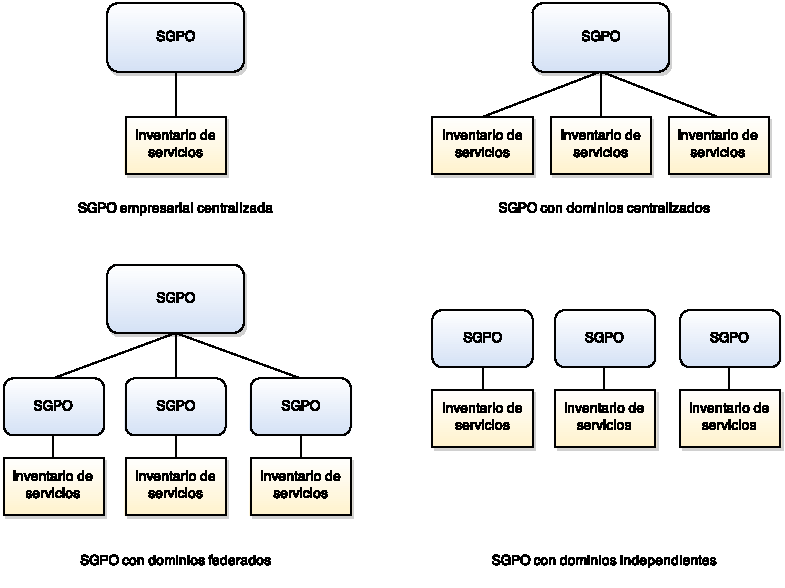
\includegraphics[width=\linewidth]{modelos_sgpo}
    \caption{Representación gráfica de modelos de jurisdicción de SGPO \cite{Erl:2011:SGG:1983453}}
    \label{imagen:modelos_sgpo}
  \end{figure}

  En el cuadro \ref{tabla:modelos_sgpo} y figura \ref{imagen:modelos_sgpo} se describen los distintos modelos de jurisdicción de SGPO básicos aplicables a una organización.

\section{Versionado}
\label{MarcoConceptual:versionado}

\section{Calidad}
\label{MarcoConceptual:calidad}

